\documentclass{article}
\usepackage[preprint]{neurips_2025}
\usepackage[T1]{fontenc}
\usepackage[utf8]{inputenc}
\usepackage{microtype,booktabs,amsmath,amssymb,graphicx}
\usepackage{tikz}
\usetikzlibrary{arrows.meta,positioning}
\usepackage[colorlinks=true,linkcolor=blue,citecolor=blue,urlcolor=blue]{hyperref}
\usepackage{url}
\title{Duplex Arena: Spatial Simulation and Trajectory Collection\ for Full-Duplex Speech Agents}
\author{Duplex Arena Project\\\url{https://github.com/KyuDan1/duplex-arena}}
\newcommand{\code}[1]{\texttt{#1}}
\begin{document}
\maketitle
\begin{abstract}
Duplex Arena connects full-duplex speech models through a shared, sample-level acoustic environment. Agents emit and receive audio concurrently, while a three-dimensional observer exposes source activity, receiver levels, propagation delays, and runtime diagnostics. The same acoustic engine supports two research workflows: frozen-model conversation inference and evaluation, and trajectory collection for reinforcement-learning integration. We describe the implemented contracts, the distinction between acoustic traces and token-policy rollouts, and bounded NVIDIA B200 experiments with PersonaPlex, Moshi, and Raon. Two 60-second PersonaPlex--Moshi experiments completed at wall-clock rate with zero dropped output samples or input overflows; recorded model inputs matched the preceding receiver blocks exactly after PCM16 encoding. Additional two- and three-agent conversations supply selected audiovisual demonstrations. These measurements establish audio routing and execution feasibility, not a semantic benchmark or a trained speech policy. We document startup buffering, recognition provenance, observed dialogue failures, and the interfaces still required for full-weight speech-model reinforcement learning.
\end{abstract}

\section{Introduction}
Full-duplex speech models receive acoustic input while generating speech. This makes their interaction difficult to evaluate with text-only, alternating-turn harnesses: a speaker can continue, backchannel, or stop while another speaker is already active. Spatial effects add another distinction. What a source emits is not what every listener hears. Distance, occlusion, reflection, and microphone noise change the acoustic evidence available to each policy.

Duplex Arena makes this interaction explicit. Independent model workers exchange audio only through a shared acoustic engine. The engine records each emitted waveform, each spatially mixed receiver waveform, and the block presented to each model adapter. A browser observes the resulting scene without controlling its clock. Completed experiments can be replayed without keeping GPUs allocated.

The project has two intended uses. In \emph{inference and evaluation}, frozen models converse under a chosen scene, and the investigator examines audio, timing, overlap, and optional recognition. In \emph{trajectory collection}, the investigator obtains aligned acoustic observations, emissions, rewards, and runtime state for analysis or a future learner. The currently implemented small REINFORCE example trains a synthetic listen/speak gate. Native speech-model inference does not expose the token probabilities needed to claim on-policy optimization of speech-language model (SLM) weights.

This report is an implementation and execution record, dated October 12, 2026, grounded in repository revision \code{4e4f0f4} and the recorded jobs identified below. It does not present a leaderboard, a new pretrained speech model, or evidence of improved task performance. Its contribution is a concrete experimental substrate and an auditable boundary between what has run and what remains to be implemented.

\section{Models and scope}
Moshi models parallel incoming and outgoing speech streams and jointly produces text and audio tokens \citep{defossez2024moshi}. PersonaPlex adds role and voice conditioning to a Moshi-derived full-duplex model \citep{roy2026personaplex}. In the arena, both are external inference workers. Their native text is retained as one evidence stream; it is never substituted for an acoustic observation. Raon is also connected through experimental bridges, with the runtime and audio-quality qualifications in Section~\ref{sec:raon}.

The current scene exposes three named slots, \code{persona}, \code{moshi}, and \code{custom}. A slot name is an identifier rather than an architectural restriction: the cafe demonstration assigns PersonaPlex to both the first and second slots. A prerecorded WAV source is supported for controlled stimulation, but it is not counted as a model participant. The three-agent showcase uses two PersonaPlex instances and one Moshi instance, hence three participants and two model families.

\section{System and acoustic contract}
\begin{figure}[t]
\centering
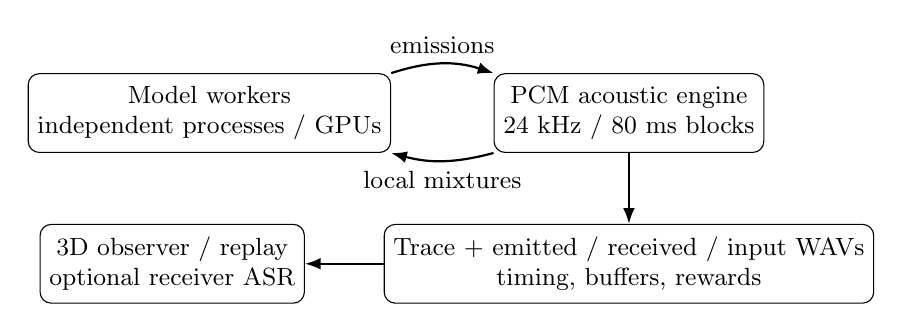
\begin{tikzpicture}[font=\small, node distance=6mm, box/.style={draw,rounded corners,align=center,minimum height=10mm},arr/.style={-{Latex[length=2mm]},thick}]
\node[box] (a) {Model workers\\independent processes / GPUs};
\node[box,right=13mm of a] (b) {PCM acoustic engine\\24 kHz / 80 ms blocks};
\node[box,below=9mm of b] (c) {Trace + emitted / received / input WAVs\\timing, buffers, rewards};
\node[box,left=10mm of c] (d) {3D observer / replay\\optional receiver ASR};
\draw[arr] (a.north east) to[bend left=18] node[above]{emissions} (b.north west);
\draw[arr] (b.south west) to[bend left=15] node[below]{local mixtures} (a.south east);
\draw[arr] (b)--(c);\draw[arr] (c)--(d);
\end{tikzpicture}
\caption{Workers listen and speak concurrently. The observer consumes recorded or live state; it does not drive acoustic time. Privileged clean source audio is available to analysis, not fed to a peer model as its observation.}
\label{fig:system}
\end{figure}

\subsection{Simultaneous actions and delayed observations}
The engine operates on mono float32 blocks with sample rate $f_s=24{,}000$ Hz and block length $B=1{,}920$, giving a decision interval $\Delta=B/f_s=80$ ms. At a boundary, each policy consumes its previous completed receiver block. All current emissions are then propagated together to produce the next observations. The initial input is silence. Missing actions in the parallel CPU environment represent silence.

Let $x_i$ be the emitted waveform of agent $i$ and $y_j$ the microphone waveform for receiver $j$. With fixed geometry within an emission event, the direct component is
\begin{align}
 g_{ij}&=\frac{1}{\max(1,d_{ij})}\prod_{k\in\mathcal{O}_{ij}}10^{-L_k/20}, &
 \tau_{ij}&=\left\lceil\frac{d_{ij}}{343}f_s\right\rceil,\\
 y_j[n]&=\sum_{i\ne j}g_{ij}x_i[n-\tau_{ij}]+r_j[n]+\epsilon_j[n].
\end{align}
Here $d_{ij}$ is Euclidean distance in meters, $L_k$ is the loss in dB of an intersected divider, and $\epsilon_j$ is independent Gaussian microphone noise with RMS $10^{\eta/20}$ for configured noise level $\eta$. There is no own-source path. Delay queues persist across block boundaries, and the ceiling prevents direct arrivals earlier than the modeled propagation time.

The optional $r_j$ term is one right-wall image-source reflection, with pressure gain $0.45\rho/\max(1,d^{\mathrm{refl}}_{ij})$ and corresponding delay. The control $\rho$ is a reflection amount, not a calibrated reverberation time. Geometry is evaluated when a block is emitted; later motion does not rewrite audio already in flight. Raw superposition remains unclipped. WAV encoding and live adapter inputs clamp to $[-1,1]$, with clipping diagnostics.

The block decision delay is distinct from physical propagation, codec buffering, and neural inference. For example, a 1 m path has approximately 2.9 ms acoustic travel time, but the peer policy still receives the preceding completed 80 ms observation block. Reporting only a propagation label or a server handler time would understate the full interaction path.

\subsection{Runtime isolation and observability}
Headless CPU simulation advances deterministically without wall-clock pacing. Live evaluation instead uses independent asynchronous send/receive loops and a paced simulation clock. Bounded worker queues expose underruns, input overflow, dropped output, and queued samples. Slow browser observers lose stale visual frames rather than delaying the acoustic loop. A fixed engine seed does not make asynchronous GPU inference bitwise reproducible.

The viewer displays transmitted and received RMS separately. Its sound rings intentionally slow apparent propagation for visibility; they are not a physical clock. Levels are dBFS rather than calibrated sound-pressure levels. Speech activity uses a $-65$ dBFS energy threshold and is not a speech recognizer. These distinctions also apply to overlap statistics: simultaneous above-threshold emissions are not automatically inappropriate interruption.

\section{Two research workflows}
\subsection{Frozen-model inference and evaluation}
The conversation launcher starts two or three native workers, assigns one job-local GPU per instance, waits for readiness, and runs a bounded evaluation. The pair launcher additionally supports a 24 kHz mono PCM16 stimulus. Each independent experiment runs in one Slurm allocation; launchers and transport ports remain local to that job. PersonaPlex and Moshi use separate Python environments because both upstream projects install a package named \code{moshi}.

For each slot, the evaluator streams three WAVs: \code{emitted} is the source signal consumed by the mixer, \code{received} is the resulting local microphone mixture, and \code{input} is the previous receiver block presented to the adapter. A JSONL trace stores per-tick scene state, signal levels, reward terms, transcripts, and worker diagnostics. The summary records completion or failure, number of frames, elapsed wall time, scheduler lateness, and final state. Failures preserve partial artifacts and are not silently labeled complete.

Replay loads those finished artifacts. It cannot modify recorded acoustics and does not reconnect to model workers. The engineering view can play a selected receiver's actual mixture. The presentation view instead plays a clean sum of participant emissions for intelligible demonstration; exported video applies loudness mastering. Consequently, a showcase soundtrack is not evidence of what any specific model heard. That evidence resides in receiver and input WAVs.

\subsection{Acoustic trajectories for learning integration}
Trajectory collection is a research workflow using the same evaluator, not a separate CLI mode. A model conversation already supplies an \emph{acoustic trajectory}: time-indexed emissions, microphone observations, geometry, proxy rewards, and diagnostics. Such traces support debugging, dataset construction, replay, and development of future reward functions. They do not reveal which model tokens were sampled or their probabilities.

The CPU interface \code{DuplexArenaEnv} provides parallel dictionaries for observations, rewards, terminations, truncations, and information. Each observation includes local microphone PCM, the agent's own position, and simulation time. It excludes other agents' clean source signals and future audio. Each action is one emitted PCM block. The fixed horizon is a truncation, not a natural task termination. This interface resembles a parallel multi-agent environment but is not registered as a PettingZoo environment.

The implemented acoustic reward combines three transparent proxies. Source-attributed delivered levels, relative to $\max(-65,\eta+6)$ dBFS, produce an audibility contribution bounded between zero and $0.10$. An active source receives $-0.04$ when more than one source is active. Emission energy contributes $-0.015(\operatorname{RMS}(x_i)/0.2)^2$. The audibility term uses source-attributed energy before noise, not recognition correctness. Penalizing all overlap can penalize useful backchannels; maximizing this reward cannot establish better dialogue.

The example \code{examples/on\_policy.py} learns a four-parameter Bernoulli gate per agent. Its features include local received RMS and time features; an active gate emits a synthetic sinusoid. Policies remain frozen throughout an episode. The trace records policy version, sampled gate, behavior log-probability, reward decomposition, and truncation. Discounted returns with $\gamma=0.97$ drive a REINFORCE-style update \citep{williams1992simple}, using a baseline from previous rollouts. This is a working policy-gradient integration example, not an SLM learner or a demonstration of learned conversational ability.

\section{B200 execution evidence}
\subsection{Environment and protocol}
The inspected server exposed NVIDIA B200 devices with 183,359 MiB each, driver 580.95.05, and driver CUDA ceiling 13.0. Timed model experiments ran in isolated Slurm jobs, with two GPUs, 16 CPU cores, and 96 GiB host RAM for the paired conversations. The worker image was NVIDIA PyTorch 25.04, providing a compiler for runtime kernel generation. Both primary model environments used Torch 2.8.0 with CUDA 12.8 wheels; the arena used a separate Python 3.13 environment.

PersonaPlex's upstream dependency metadata pins an older Torch version, and its reused environment had unrelated package conflicts. The measurements validate the exercised inference path, not a clean dependency resolution for every installed package. Moshi's independent environment passed its dependency check. Exact source/checkpoint revisions and operational details are recorded in \href{https://github.com/KyuDan1/duplex-arena/blob/main/docs/B200_VERIFICATION.md}{the B200 execution record}.

Two primary experiments used the same spoken rice-cooking stimulus, derived from PersonaPlex's example WAV and converted to the arena format. The stimulus occupied the third slot, with spoken intervals around 4.08--8.56 s and 22.64--26.88 s. Each experiment ran for 750 frames (60 s). The near condition used 1 m model separation, no divider, and $-72$ dBFS noise. The distant condition used 5.70 m separation, a 14 dB divider, and $-35$ dBFS noise. The conditions change several factors together and are not an acoustic ablation.

\begin{table}[t]
\centering
\caption{Bounded PersonaPlex--Moshi experiments. Timing is measured after startup. Underruns are startup frames; no prefill was used. Overlap duration counts the two models only.}
\label{tab:pair}
\begin{tabular}{lrr}\toprule
Measurement & Near / quiet & Distant / cocktail\\\midrule
Slurm job & 189794 & 189798\\
Audio / wall duration (s) & 60 / 60.011 & 60 / 60.007\\
Scheduler lateness, p95 (ms) & 1.45 & 2.04\\
Tick deadline overruns & 0 & 0\\
Input overflow / dropped samples & 0 / 0 & 0 / 0\\
PersonaPlex / Moshi underrun frames & 1 / 2 & 1 / 2\\
Moshi handler mean / p95 (ms) & 24.59 / 26.15 & 24.19 / 26.20\\
Both models active (s) & 3.12 & 6.56\\
Direct path pressure gain (dB) & 0 & $-29.12$\\\bottomrule
\end{tabular}
\end{table}

\subsection{Routing, timing, and memory}
For every receiver in both paired runs, the saved input block at tick $t$ matched the PCM16 encoding of the received block at $t-1$ exactly, with an initial silent input. Re-rendering recorded source WAVs through the mixer reproduced received audio to maximum normalized amplitude errors of $9.2\times10^{-5}$ and $4.5\times10^{-5}$ for near and distant runs, respectively. Small differences arise from recording quantization. These checks establish the intended route into the adapter; native transport encoding remains a separate codec stage.

Table~\ref{tab:pair} shows wall-clock completion and scheduler diagnostics. Startup underruns occurred before model output arrived, and one queued 80 ms block remained at the fixed episode boundary. No ADC or Opus-decoder clipping was counted. Moshi handler times measure the server's frame-processing scope, not end-to-end response latency.

A one-minute monitoring window during the near run reported approximately 17,839 MiB for Moshi and 19,625 MiB for PersonaPlex, with about 36.4 GiB host working memory and no OOM or CPU-throttling events. These are sampled monitoring-window readings, not exact allocator peaks. They should not be reused as optimizer-state estimates for training.

Offline Whisper recognition \citep{radford2023whisper} found cooking-answer content in PersonaPlex's received audio and PersonaPlex speech in Moshi's received audio. The second stimulus began while Moshi was active; overlap and subsequent stopping/resuming were visible. This establishes an interruption stimulus and response activity, not a causal measure of intentional yielding. Noisy receiver recognition also contained hallucinated repetitions. Neither ASR nor model-generated text is treated as ground-truth comprehension.

\subsection{Two- and three-agent demonstrations}
\begin{table}[t]
\centering
\caption{Additional conversations used for selected audiovisual examples. Every model occupied a separate B200. Each run had zero input overflow, output drops, and clipping.}
\label{tab:showcase}
\begin{tabular}{lrrr}\toprule
 & Friends & Clerk / customer & Three agents\\\midrule
PersonaPlex / Moshi instances & 1 / 1 & 2 / 0 & 2 / 1\\
Slurm job & 189846 & 189891 & 189845\\
Full recording (s) & 90 & 60 & 90\\
Scheduler lateness, p95 (ms) & 1.57 & 1.69 & 1.26\\
Startup underrun frames & 1 + 2 & 1 + 1 & 1 + 2 + 1\\
Selected interval (s) & 0--26.92 & 9.50--30.25 & 0--14.92\\\bottomrule
\end{tabular}
\end{table}

The conversations in Table~\ref{tab:showcase} have no prerecorded speaker. In the cafe run, PersonaPlex workers receive clerk/customer roles, voice prompts, and menu context; their dialogue lines are not scripted. The selected passage contains an iced oat-latte and croissant order and confirmation. The full recording also includes initial customer/clerk role confusion and an incorrect price, excluded from the selected clip. Longer friends and three-agent recordings include monologues and repetitive backchannels. Selection makes the examples useful for presentation but introduces clear selection bias.

Full-run model overlap was 10.96 s for the friends run and 48.08 s for the three-agent run; selected intervals contain 3.76 s and 6.96 s, respectively. These are activity measurements, not quality scores. Every connected model's recorded input matched its preceding receiver block. The presentation uses a slowly rotating 3D camera, word-timed speech bubbles, activity lanes, and timing counters. Bubbles derive from \emph{offline Whisper-small on emitted audio}, revealed at word timestamps. Their streaming appearance is not a measurement of online ASR latency.

\subsection{Raon: transport feasibility with unresolved quality}\label{sec:raon}
The direct Raon PyTorch bridge produced actual text and audio but averaged 207 ms per 80 ms frame. Its 32-frame input queue filled after 4.24 simulated seconds, and job 189796 failed while preserving a partial trace. The worker reported about 19.4 GiB peak PyTorch allocation. This bridge did not meet real-time requirements.

An optimized SGLang path required an isolated CUDA 13 runtime overlay and library-path correction. Job 189820 subsequently completed 60 s in 60.012 wall seconds, with 1.68 ms p95 scheduler lateness, zero input overflow/output drops, and no clock overruns. Raon had six startup underrun frames and 480 ms queued at episode end. Monitoring reported about 90,085 MiB for Raon and 19,697 MiB for PersonaPlex; the larger Raon footprint includes SGLang's preallocated cache.

Successful transport did not imply clean synthesis. Warmup encountered a mask/embedding mismatch and fell back; the loader also warned that the SDPA Mimi fallback lacked intended sliding-window behavior. Later emitted audio substantially diverged from generated text and contained garbled phrases. These are candidate implementation causes, not proven causal explanations. Raon was therefore excluded from the showcase and is not certified here for long-form audio quality.

\section{From acoustic traces to SLM reinforcement learning}
A gradient-capable learner needs model actions, not an ASR reconstruction of speech. The next interface must expose episode and agent identifiers, checkpoint revision, policy version, sampling configuration, input sample interval, sampled text/audio-code token IDs, token positions, behavior log-probabilities, valid-action masks, and token-to-emitted-sample alignment. Value estimates are needed when the selected learner uses a critic. Reset boundaries, recurrent/KV state, and truncation versus termination must also be explicit.

A defensible implementation sequence is:
\begin{enumerate}
\item Instrument one frozen model and recompute logged behavior probabilities under identical weights, history, masks, and sampling transforms. Temperature or top-$k$ changes must be reflected in the distribution being logged.
\item Add policy-version barriers. Finish or discard version-$v$ episodes before publishing version $v+1$, reset model state, and acknowledge the new version before collecting its actions. Pausing a socket is insufficient.
\item Align acoustic rewards and advantages to sampled tokens, including delayed propagation and truncated episodes. Keep privileged critic state separate from each actor's microphone observation.
\item Validate a bounded adapter/LoRA update with finite gradients, checkpoint/resume, and reference-policy controls before considering full-weight distributed optimization.
\item Evaluate a frozen baseline and updated policy on held-out, labeled tasks with repeated seeds and controlled stimuli. Measure intelligibility, task success, turn timing, and interruption recovery separately.
\end{enumerate}
The existing REINFORCE gate supplies a small example of frozen-policy rollout bookkeeping. It does not satisfy these model-internal contracts. Full-weight SLM RL remains future work, and no learning curves or trained-model improvements are claimed.

\section{Limitations, reproducibility, and responsible use}
The acoustic engine is intentionally simple: three slots, quadratic source--receiver paths, a single reflection, nondirectional sources/microphones, and no validated room impulse response or HRTF. It models neither calibrated SPL nor a physical loudspeaker--microphone feedback loop. A more realistic environment should validate measured or richer simulated impulse responses before using spatial outcomes as perceptual predictions.

The execution evidence consists of a small number of bounded episodes with stochastic models. It lacks repeated-seed confidence intervals, human intelligibility labels, and controlled counterfactual interruption trials. Changed acoustic conditions also alter downstream model actions, preventing isolated attribution to distance, noise, or occlusion. Selected videos cannot substitute for full-run evaluation. Low scheduler lateness and zero dropped buffers establish engineering behavior rather than language understanding.

Re-execution requires independent model environments, authorized local model weights, and the documented GPU launchers. Local credentials, private paths, model weights, and large recordings are excluded from version control. The public repository includes generic configurations, the acoustic and evaluation code, tests, the replay renderer, and this report. Relevant source entry points are \code{acoustics.py}, \code{engine.py}, \code{evaluation.py}, \code{env.py}, and \code{examples/on\_policy.py}; detailed commands are maintained in the README and GPU/server documentation.

Audio conditioning and generated speech must respect model licenses and voice permissions. Label generated audio and caption provenance. A plausible transcript or confident synthetic voice does not establish factual correctness, as the cafe price error illustrates. Retain unselected trajectories and failure summaries alongside curated media so that favorable examples do not erase observed failures.

\bibliographystyle{plainnat}
\bibliography{duplex-arena-technical-report}
\end{document}
